\section{Research Goals}
\label{problem}

The design of the Internet and routing protocols have no notion of national borders, and thus Internet traffic paths are determined without any regard to international crossings.  Issues arise when Internet traffic flows through countries which have different data privacy and surveillance laws; which geographic locations does one traffic flow pass through and which laws should govern it?  The BGP (Border Gateway Protocol) decides interdomain routing paths based on shortest and most preferred paths - not on which countries it will traverse.  This allows traffic to pass through countries that conduct surveillance even when the traffic originates (and possibly terminates) in a country that does not lawfully allow surveillance.  

Determining where a client's Internet traffic flows is complicated by the complexity of websites~\cite{butkiewicz2011understanding}.  Many websites also fetch content from other domains, which are most likely hosted in different locations.  Therefore, the client has to make additional web requests, which take different paths.  One initial web request can result in content being fetched from many servers located around the world, and to see where this traffic flows requires knowledge of all paths from the client to requested sources (and all the requested sources to the client).  Figure~\ref{fig:domains} shows the number of subsequent requests that are made from an initial web request for the Brazilian Alexa Top 100 domains.  As the number of domains, and therefore the number of paths, increase, the more possibilities for surveillance are introduced.

\begin{figure}
\centering
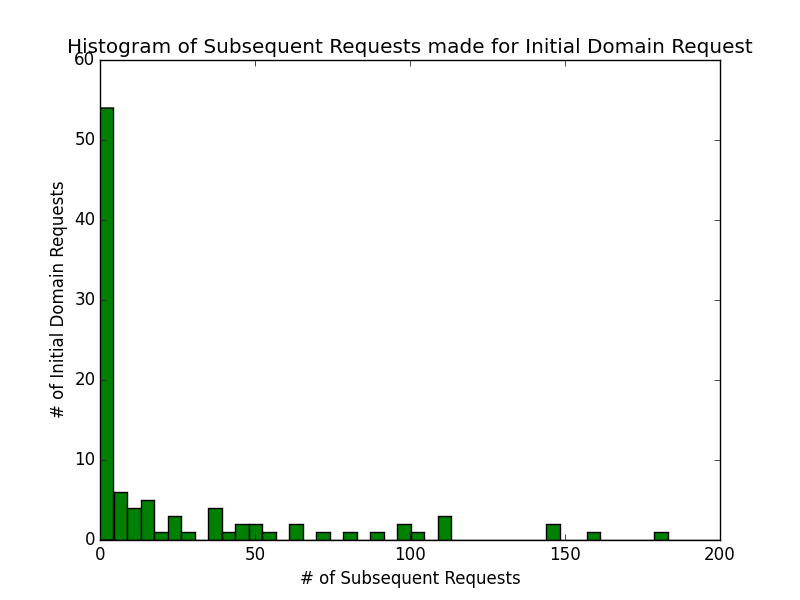
\includegraphics[width=.5\textwidth]{subsequent_request_hist}
\caption{A histogram of the number of third party requests are made by each initial domain request for the Brazilian Alexa Top 100 domains.}
\label{fig:domains}
\end{figure}

\begin{thm}
Measure how much Internet traffic traverses countries that are known for surveillance, and quantify how much possible surveillance can be conducted.  Use Brazil as a case study by measuring the country-level routing paths for clients in Brazil to the Brazilian Alexa Top 100 domains (and the subsequent domain requests); collect data on how much traffic is solely transmitted by countries that conduct surveillance and how much traffic has a destination in one of these countries.
\end{thm}

There are naive ways for clients to force their traffic to avoid potential surveillance.  One way is using EDNS (Extension mechanisms for DNS); a client could spoof his own client subnet in the DNS request, such that it appears as if the client is located in a geographically different location.  This different location could potentially be closer to a georeplicated server in a foreign country, and thus the path from the server to the client has a greater likelihood of avoiding certain countries.  The same method could be used with open resolvers in geographically different locations.  Figure~\ref{fig:resolvers} shows a scenario where this method would help clients avoid a country.  Unfortunately, this approach is unsuccessful if the service uses anycast IP addresses; this technique has increased in the past few years~\cite{cicalese2015characterizing}.  IP anycast is the case where a set of servers share the same standard unicast IP address, despite being in geographically diverse locations.  Even though the DNS lookup is in a different location than the client, the client will still be accessing data from the server that is closest, which provides the possibility of unwanted countries on the path between the server and the client.  

\begin{figure*}
\centering
\begin{subfigure}[t]{.5\textwidth}
  \centering
  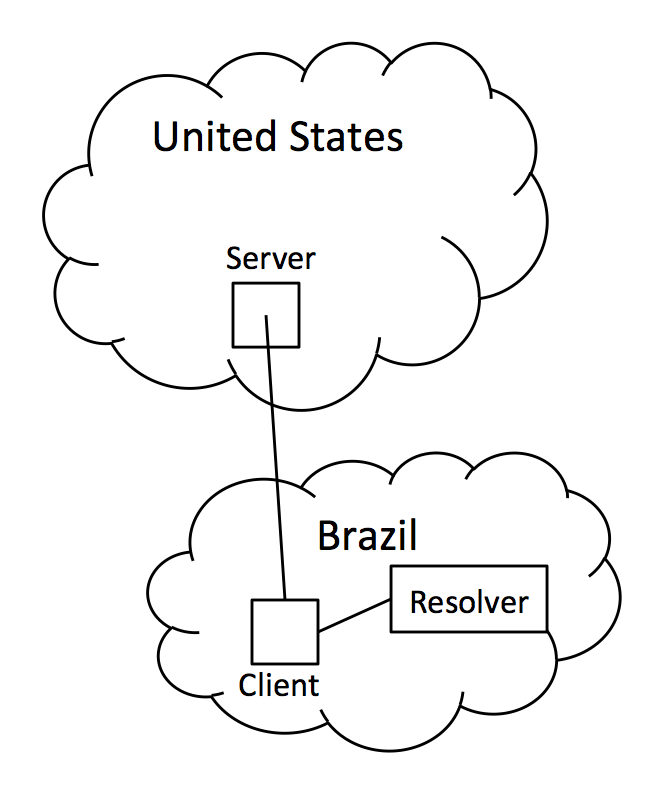
\includegraphics[width=.4\linewidth]{no_open_resolver}
  \caption{A possible path when a client uses a local resolver.}
  \label{fig:local_resolver}
\end{subfigure}%
\begin{subfigure}[t]{.5\textwidth}
  \centering
  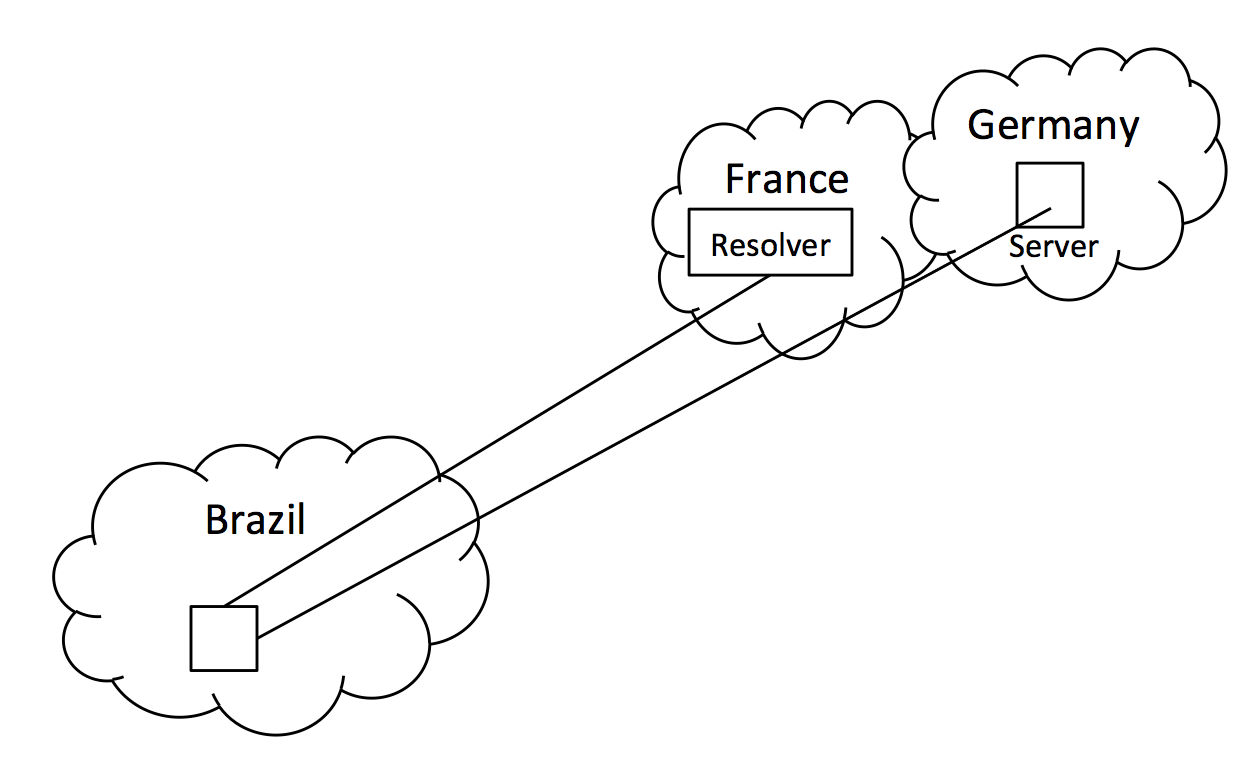
\includegraphics[width=.7\linewidth]{open_resolver}
  \caption{A possible path when a client uses an open resolver in a geographically different location.}
  \label{fig:open_resolver}
\end{subfigure}%
\caption{Different paths are shown when a client uses a local resolver (Figure~\ref{fig:local_resolver}) vs. a geographically distant open resolver (Figure~\ref{fig:open_resolver}.)}
\label{fig:resolvers}
\end{figure*}

\begin{thm}
Design and implement a system that allows clients to avoid countries known for surveillance.  The system should be resistant to the use of IP anycast, and should take into account the subsequent requests made when fetching a webpage.
\end{thm}

\begin{thm}
Evaluate the country avoidance system for how well it can avoid any given country for any given (client, server) pair.  Quantify how much surveillance protection this system provides as compared to clients not using the system.
\end{thm}
